
 \documentclass[12pt]{article}
\usepackage{graphicx}
\usepackage{booktabs}
 \usepackage{makecell}
 \usepackage{float}
 \newcommand{\diff}{\,\mathrm{d}}
\usepackage[margin=1in]{geometry}
\usepackage{fancyhdr}
\pagestyle{fancy}
\usepackage{extarrows}
\usepackage{breqn}

\newcommand{\N}{\mathbb{N}}
\newcommand{\Z}{\mathbb{Z}}
\newcommand{\trans}{^{\mathrm T}}
\usepackage{amssymb}
\usepackage[table]{xcolor}
\usepackage{bm}
\usepackage{array}
\usepackage{mathtools}
\usepackage[english]{babel}
\usepackage{natbib}
\usepackage{url}
\usepackage[utf8x]{inputenc}
\usepackage{amsmath}
\usepackage{graphicx}
\graphicspath{{images/}}
\usepackage{parskip}
\usepackage{fancyhdr}
\usepackage{vmargin}
\usepackage[font={bf, footnotesize}, textfont=md]{caption}
\usepackage{amsmath,amsthm,amssymb}


\newenvironment{theorem}[2][Theorem]{\begin{trivlist}
\item[\hskip \labelsep {\bfseries #1}\hskip \labelsep {\bfseries #2.}]}{\end{trivlist}}
\newenvironment{lemma}[2][Lemma]{\begin{trivlist}
\item[\hskip \labelsep {\bfseries #1}\hskip \labelsep {\bfseries #2.}]}{\end{trivlist}}
\newenvironment{exercise}[2][Exercise]{\begin{trivlist}
\item[\hskip \labelsep {\bfseries #1}\hskip \labelsep {\bfseries #2.}]}{\end{trivlist}}
\newenvironment{reflection}[2][Reflection]{\begin{trivlist}
\item[\hskip \labelsep {\bfseries #1}\hskip \labelsep {\bfseries #2.}]}{\end{trivlist}}
\newenvironment{proposition}[2][Proposition]{\begin{trivlist}
\item[\hskip \labelsep {\bfseries #1}\hskip \labelsep {\bfseries #2.}]}{\end{trivlist}}
\newenvironment{corollary}[2][Corollary]{\begin{trivlist}
\item[\hskip \labelsep {\bfseries #1}\hskip \labelsep {\bfseries #2.}]}{\end{trivlist}}
\DeclareMathOperator{\tr}{tr}
\DeclareMathOperator{\rank}{rank}
\DeclareMathOperator{\Span}{span}
\DeclareMathOperator{\row}{row}
\DeclareMathOperator{\col}{col}
\DeclareMathOperator{\range}{range}
\DeclarePairedDelimiterX{\inp}[2]{\langle}{\rangle}{#1, #2}
\DeclareMathOperator{\Proj}{Proj}
\DeclareMathOperator{\trace}{trace}
\newcommand{\Her}{^{\mathrm H}}
\DeclareMathOperator{\diag}{diag}
\makeatletter 
    \newcommand\fcaption{\def\@captype{table}\caption}
\makeatother
\setmarginsrb{3 cm}{2.5 cm}{3 cm}{2.5 cm}{1 cm}{1.5 cm}{1 cm}{1.5 cm}
\setlength\parindent{1em}

\title{Short Report: Large Amplitude Pendulum}                             % Title
\author{Chen Ang}                               % Author
\date{\today}                                           % Date

\makeatletter
\let\thetitle\@title
\let\theauthor\@author
\let\thedate\@date
\makeatother

\pagestyle{fancy}
\fancyhf{}
\rhead{\theauthor}
\lhead{\thetitle}
\cfoot{\thepage}

\begin{document}

%%%%%%%%%%%%%%%%%%%%%%%%%%%%%%%%%%%%%%%%%%%%%%%%%%%%%%%%%%%%%%%%%%%%%%%%%%%%%%%%%%%%%%%%%

\begin{titlepage}
    \centering
    \vspace*{0.5 cm}
    
\includegraphics[scale = 0.75,width=6cm]{CUHK}\\[1.0 cm]   % University Logo
    \textsc{\large The Chinese University of Hong Kong, Shenzhen}\\[2.0 cm]   % University Name
    \textsc{\Large PHY 1002}\\[0.5 cm]               % Course Code
    \textsc{\large Physics Laboratory}\\[0.5 cm]               % Course Name
    \rule{\linewidth}{0.2 mm} \\[0.4 cm]
    { \huge \bfseries \thetitle}\\
    \rule{\linewidth}{0.2 mm} \\[1.5 cm]
    
    \begin{minipage}{0.4\textwidth}
        \begin{flushleft} \large
            \emph{Author:}\\
            \theauthor
            \\
            \emph{Group Number:} \\
            Group 1
            \end{flushleft}
            \end{minipage}~
            \begin{minipage}{0.4\textwidth}
            \begin{flushright} \large
            \emph{Student Number:} \\
            118010009                                   % Your Student Number
            \\
            \emph{Experiment Date:}\\
            September 27, 2019
        \end{flushright}
    \end{minipage}\\[2 cm]
    
    {\large \thedate}\\[2 cm]
 
    \vfill
    
\end{titlepage}

%%%%%%%%%%%%%%%%%%%%%%%%%%%%%%%%%%%%%%%%%%%%%%%%%%%%%%%%%%%%%%%%%%%%%%%%%%%%%%%%%%%%%%%%%
%%%%%%%%%%%%%%%%%%%%%%%%%%%%%%%%%%%%%%%%%%%%%%%%%%%%%%%%%%%%%%%%%%%%%%%%%%%%%%%%%%%%%%%%%

\tableofcontents
\pagebreak


%%%%%%%%%%%%%%%%%%%%%%%%%%%%%%%%%%%%%%%%%%%%%%%%%%%%%%%%%%%%%%%%%%%%%%%%%%%%%%%%%%%%%%%%%

\rmfamily

\section{Rectangular Bar Pendulum: Minimum Period}
\subsection{$x-T$ Plot}

\begin{figure}[H]
	\centering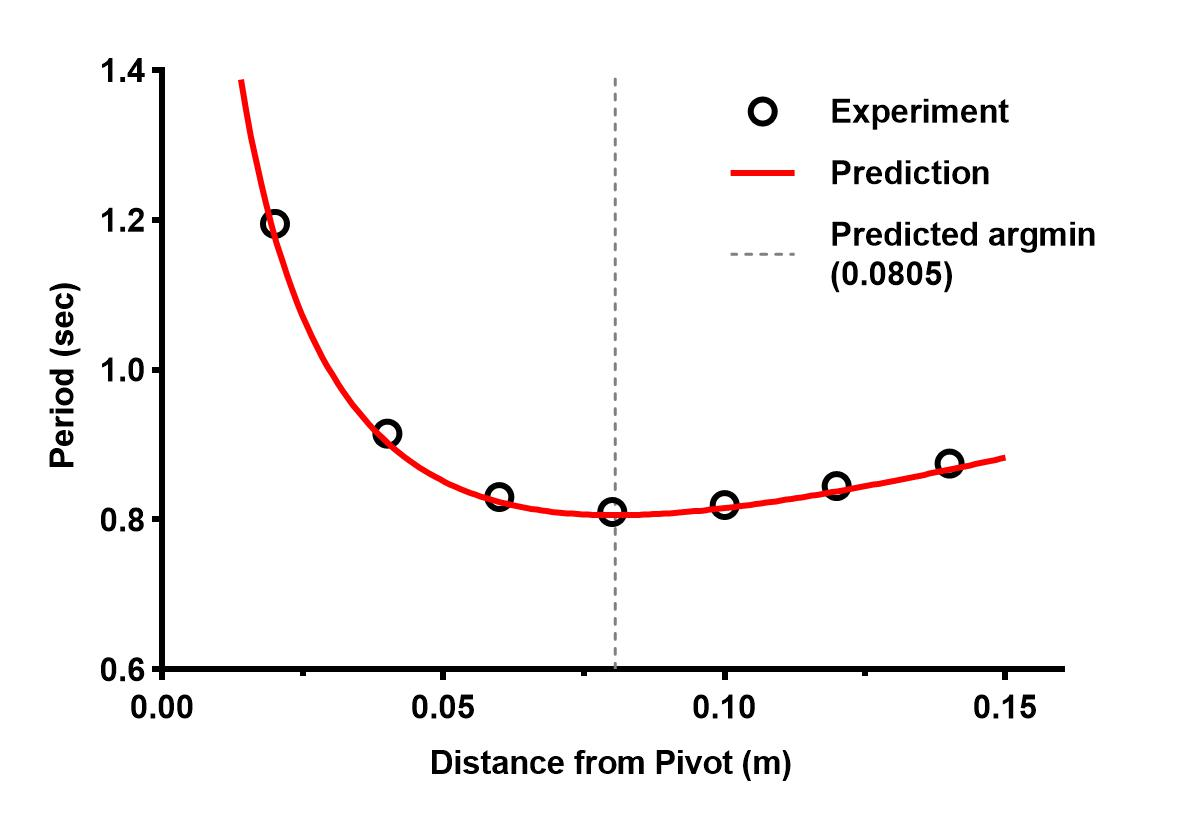
\includegraphics[width=10cm]{icm1}
	\caption{Relationship of pivot-CM distance $x$ and period of the pendulum $T$ }
	\label{$Frequency-Intensity$ Graph for $70$cm tube}
\end{figure}

\subsection{Minimum Period}

The following table records $x_0$ ($x$ that gives the minimum period) and $T_{\text{min}}$, obtained both from the experiment and theory. The percentage differences of the experimental values from predictions are calculated for comparison.\\


\begin{table}[!htb]
\centering
\begin{tabular}{|c|c|c|c|}
	\hline 
	& Experiment & Prediction & Relative Difference \\ 
	\hline 
	$x_0$ (cm) & 8.00 & 8.05 & $-0.62\%$ \\ 
	\hline 
	$T_{\text{min}}$ (s) & 0.810 & 0.807 & $+0.37\%$ \\ 
	\hline 
\end{tabular}
\caption{Values of $x_0$ and corresponding minimum period $T_{\text{min}}$}
\end{table}

The experimental values fit well with our theory.
 
\section{Rotational Inertia of a Disk}
\subsection{Raw Data}
$$T=0.494\pm0.001\text{ s}$$
$$M=89.37\pm0.02\text{ g}$$
$$d=R=4.0\pm0.1\text{ cm}$$
$$g=9.78\pm0.01\text{ N}\cdot \text{kg}^{-1}$$

\subsection{Rotational Inertia about CM}
The experimental value of rotational inertia about CM is given by
$$I_{\text{exp}}=
\frac{T^2Mgd}{4\pi^2}-Md^2=(7.31\pm 0.20) \times 10^{-5}\text{ kg}\cdot \text{m}^{2}
$$
and the theoretical value given by
$$I_{\text{theo}}=\frac12MR^2=(7.15\pm 0.36) \times 10^{-5}\text{ kg}\cdot \text{m}^{2}
$$
with a relative difference of
$$\frac{I_{\text{exp}}-I_{\text{theo}}}{I_{\text{theo}}}=2.24 \ \%$$


\section{Rotational Inertia of an Irregular Pendulum}
\subsection{Raw Data}
$$M=10.07\pm0.02\text{ g}$$
$$r=1.4\pm0.1\text{ cm}$$
$$g=9.78\pm0.01\text{ N}\cdot \text{kg}^{-1}$$
\subsection{$t-\omega$ Plot and $I_{\text{CM}}$ of the Irregular Pendulum}
\begin{figure}[H]
	\centering\includegraphics[width=10cm]{icm2}
	\caption{Relationship of angular velocity $\omega$ and time $t$ }
	\label{$Frequency-Intensity$ Graph for $70$cm tube}
\end{figure}

A linear regression of the $t-\omega$ curve during one period of acceleration yields
$$\alpha=|\dot{\omega}|=22.53\pm0.04\text{ rad}\cdot\text{s}^{-2}$$
The rotational inertia of the irregular pendulum about its CM can be found, via
$$I_{\text{CM}}=Mr(\frac{g}{\alpha}-r)=(5.92\pm0.41)\times 10^{-5}\text{ kg}\cdot \text{m}^{2}$$
\end{document}
